\section{Overview}
\label{sec:rvos_overview}
Given an image $I \in \mathbb{R}^{H \times W \times 3}$ and a referring expression $T$ with $L$ words, where $H$ and $W$ are the height and the width of the image, respectively. We propose an efficient and simple end-to-end framework named VLFormer for referring image segmentation, as shown in Figure \ref{fig:VLFormer}. It consists of three main components: Backbone, Cross-modal Pixel Decoder, and Visual-Linguistic Transformer. 

% Given a video clip $V = \{V_1, V_2, ..., V_T\}$ and a referring expression with $L$ words. We propose an efficient and simple end-to-end framework named VLFormer for referring video object segmentation, as shown in Figure \ref{fig:VLFormer}. It consists of 3 main components: Backbone, Cross-modal Pixel Decoder and Transformer Decoder. 

In summary, our method can be described as follows. Each object query represents its appearance. We update the object queries by incorporating the linguistic and visual features through multiple Visual-Linguistic Transformer layers, and the final query features will be associated with the final pixel-level embedding to generate the corresponding segmentation map.   

In detail, the data flow is as follows. A backbone includes Visual Encoder and Text Encoder, which extract low-resolution feature maps from video frames and linguistic features from the corresponding referring expression, respectively. A Cross-modal Pixel Decoder incorporates low-resolution features from the backbone and linguistic features by a Language Guided Module (LGM) and upsamples these features to generate the high-resolution per-pixel embeddings. A Visual-Linguistic Transformer operates on linguistics and multi-scale visual features from the Cross-modal Pixel Decoder to process the object queries. The final binary mask predictions are generated by associating the per-pixel embeddings and object queries. We select the query with the highest confidence score as the target object during inference. 

We also extend our work to the video easily since our framework can segment and track objects naturally due to linking the corresponding queries across frames. Regarding refinement and re-tracking the target object, we use an off-the-shelf semi-supervised VOS model named STCN \cite{cheng_rethinking_2021} that uses some reference frames as a memory bank to predict the entire video.

Experiments show that our proposed network achieves competitive results in several datasets. The main contributions is as follows:
\begin{itemize}
    \item We propose VLFormer, a query-based referring image segmentation framework that efficiently interacts among multi-modal features via a Transformer-based module.
    \item We design a Visual-Linguistic Transformer Block, which associates visual and linguistic features with the object queries to produce a more fine-grained representation of object queries. 
    \item We suggest utilizing the cross-modal knowledge of the CLIP model for achieving better vision-language fusion.
    \item We achieve state-of-the-art performance on standard benchmarks such as referring image segmentation (RefCOCO/RefCOCO+) and promising results on referring video object segmentation dataset(Ref-YoutubeVOS).
\end{itemize}

\begin{figure}[H]
    \centering
    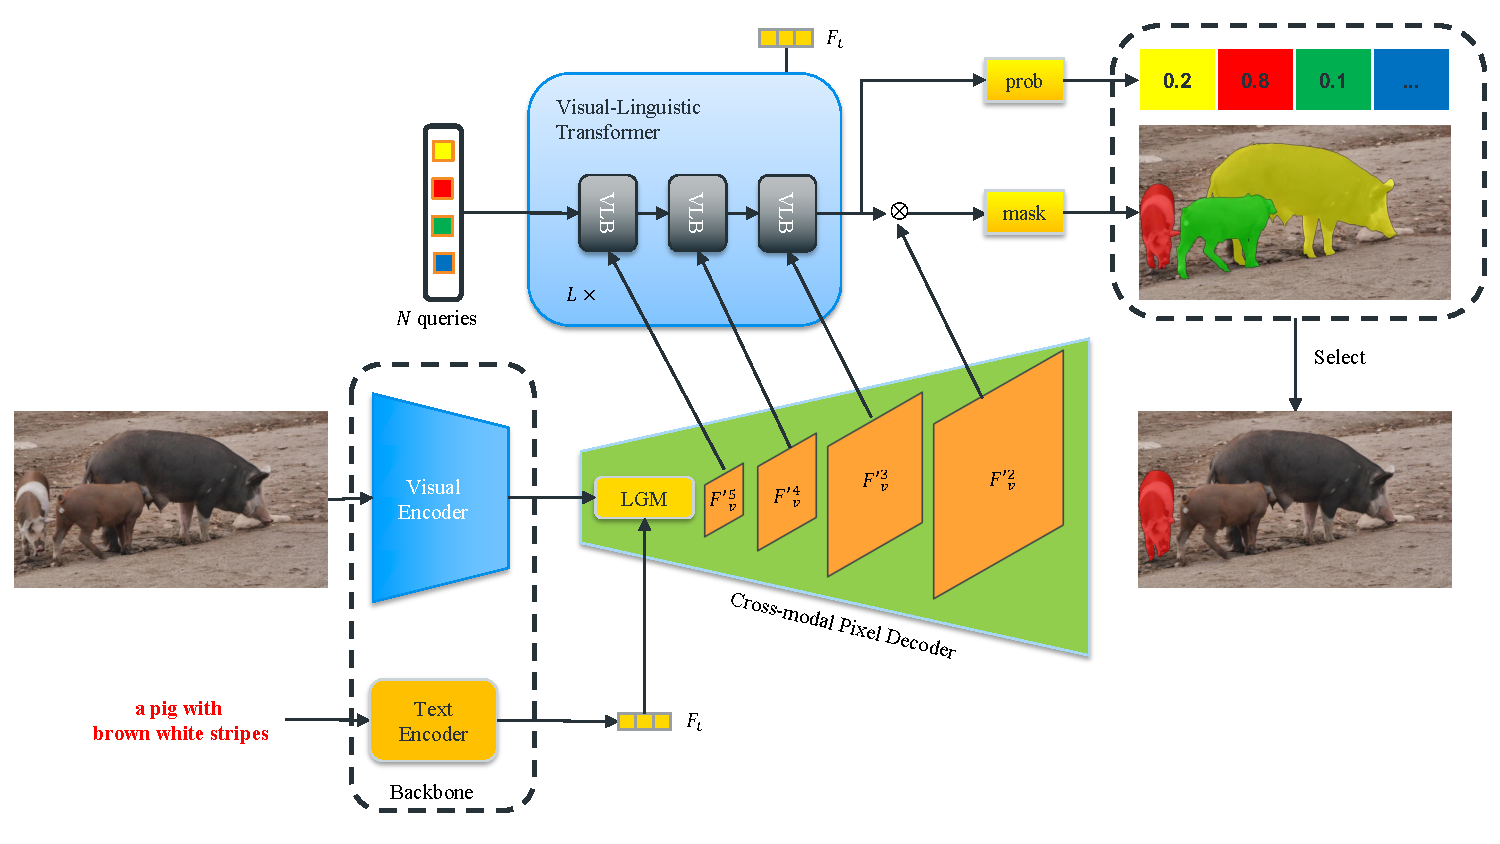
\includegraphics[width=\textwidth]{content/resources/images/referring_segmentation/NewVLFormer.pdf}
    \caption{The overview of our method VLFormer. It contains three major components: Backbone (includes Visual Encoder and Text Encoder), Cross-modal Pixel Decoder, and Visual-Linguistic Transformer. First, the model extracts visual features and linguistic features from a given image and language expression by the backbone. The visual features are then processed by a Cross-modal Pixel Decoder to generate fine-grained language-guided visual features. $N$ object queries are gradually updated by the Visual-Linguistic Transformer and then are multiplied with per-pixel embedding to output $N$ potential objects. The final object is selected based on the probability generated by the object queries.}
    \label{fig:VLFormer}
\end{figure}